\section{Zooming in on star formation} 
\label{sec:cloudtodisc}

Having described the macro-evolution of the CMZ and the present-day distribution of gas and stars in \S\ref{sec:macroevolution}, we now  zoom in on individual regions of current and future star formation in the CMZ, from cloud ($\sim10$\,pc) to protostellar ($<1000$\,au) scales. In \S \ref{sec:extremeclouds} we discuss how global processes in the CMZ result in a population of molecular clouds with extreme properties, which provide the best Galactic analogues to high-redshift star-forming regions. In \S \ref{sec:sfinaction} we explore the growing body of work dedicated to identifying and characterising the incipient and current sites of star formation throughout the CMZ, and how the environmental conditions in the CMZ may inhibit the formation of compact substructures\index{interstellar medium!molecular clouds!structure} within these clouds\index{interstellar medium!molecular clouds}.

\subsection{The extreme conditions in CMZ clouds}
\label{sec:extremeclouds}
The CMZ contains $\sim2\mhyphen6\times10^{7}$ \msun of gas at high density, yet the majority of this gas is not forming stars (\S\ref{sec:global}).  
As we expect to find star formation in the highest density gas, one of the key open questions about the CMZ is: Why is the dense gas forming stars inefficiently?

There are several ways in which molecular gas in the CMZ is qualitatively different from that in the rest of the Galaxy (Table \ref{tab:properties_overview}).
We summarise the significant effort that has been made to understand the global properties of the cloud population in the CMZ in this section.

\subsubsection{Observations at cloud scales}

Observations of star-forming gas are best done at far-infrared to millimetre wavelengths.
We begin by summarising these observations, and then describe some of their key results.
Many of the data sets mentioned in this section are publicly available and are indexed on the \href{https://github.com/CentralMolecularZone/DataSets}{CMZ Data Sets github repository}.

A number of continuum surveys targeting the CMZ have been conducted at far-IR to mm wavelengths, including the APEX Telescope Large Area Survey of the Galaxy \citep[ATLASGAL,][]{Schuller2009}, the Bolocam Galactic Plane Survey \citep[BGPS,][]{Bally2010, Rosolowsky2010, Aguirre2011, Ginsburg2013}, the Herschel Infrared Galactic Plane Survey \citep[Hi-GAL,][]{Molinari2010, Molinari2011}, the JCMT SCUBA-2 Galactic Centre Survey \citep{Parsons2018}, the IRAM-GISMO survey \citep{Arendt2019,Staguhn2019}, the MUSTANG Galactic Plane Survey \citep{Ginsburg2020}, the CARMA CMZ survey \citep{Pound2018}, the SMA CMZoom survey \citep{Battersby2020}, and the AzTEC survey of the CMZ \citep{Tang2021a, Tang2021b}.

These surveys achieve angular resolutions ranging from $3\mhyphen40^{\prime\prime}$, corresponding to physical scales $\sim0.1\mhyphen1.6$~pc. As they sample from the far-IR to mm wavelengths, the dust spectral energy distribution (SED) can be modelled to constrain the column density ($N_{\rm H_{2}}$), dust temperature ($T_d$), and opacity index ($\beta$) (see e.g. \citealt{Battersby2011, Molinari2011,Marsh2016,Tang2021a, Tang2021b} for details).  Typical column densities towards the CMZ clouds are $\sim$ 10$^{23}$~cm$^{-2}$, peaking at $>10^{24}$~cm$^{-2}$ towards Sgr B2. The cloud dust temperatures range from $\sim20\mhyphen25$~K, showing an inverse correlation with column density, with the lowest temperatures found towards the densest parts of the clouds. \citet{Tang2021a} report a dust opacity index $\beta$ in the range $1.8\mhyphen2.4$, which is steeper than seen in local clouds, even those contained within the field of view of the same CMZ data set.  The steeper index hints that dust properties in the CMZ may be fundamentally different than those in the rest of the Galaxy, which affects observational inferences at all wavelengths.

There have also been a number of molecular line surveys targeting the CMZ, including the H$_{2}$O southern Galactic Plane Survey \citep[HOPS,][]{Walsh2008, Walsh2011, Purcell2012, Longmore2017, Akhter2021}, which includes water maser and NH$_3$ observations at $\sim2.5\arcmin$ resolution, the ASTE [{C{\sc i}\xspace}] survey at 0.7mm and 34$\arcsec$ resolution \citep{Tanaka2011}, the MOPRA CMZ survey \citep{Jones2012, Jones2013} covering many lines in the 3mm band with $\sim$arcminute resolution, the APEX CMZ survey \citep{Ginsburg2016} covering H$_2$CO and $^{13}$CO in the 1.4mm band, the Survey of Water and Ammonia in the Galactic Centre \citep[SWAG,][]{Krieger2017} observing NH$_3$ and H$_2$O at $\sim30\arcsec$ resolution, and Nobeyama Radio Observatory surveys \citep{Tanaka2018,Tanaka2020} that cover many bands and transitions, particularly of HCN and HCO+.   Several surveys cover a range of CO transitions, including recent CO 3-2 observations with JCMT \citep{Parsons2018,Eden2020} at 15\arcsec resolution and many previous surveys at coarser resolution.

These extensive surveys, along with higher angular resolution follow-up observations, have led to the following important discoveries about CMZ gas density, velocity, temperature, and chemistry.

\paragraph{Molecular gas in the CMZ is denser on parsec scales than in the rest of the Galaxy:}\label{subsubsec:densitystructure}\index{interstellar medium!structure}\index{interstellar medium!molecular clouds!structure}
Dust mass measurements yield average volume densities for all dust ridge clouds comparable to cluster-forming regions in the Galactic disc \citep{Walker2015,Walker2016}.
The masses of the molecular clouds in the CMZ range from $\sim$ 10$^{4\mhyphen5}$~M$_{\odot}$ in the dust ridge and the 20/50 km~s$^{-1}$ clouds, to \textgreater \ 10$^{6}$~M$_{\odot}$ in the most extreme case of Sgr B2 \citep[e.g.][]{Immer2012b,Kauffmann2017a}.
The clouds are very compact, with typical radii of a few parsecs.
Under a simplistic assumption of spherical symmetry and uniform distribution, this translates to volume densities $>10^{4}$ \percc for all of the prominent molecular clouds in the CMZ. 

Molecular line observations confirm these high inferred densities.
Studies using multiple transitions of molecular species that are not in local thermodynamic equilibrium (LTE) have been used to measure local volume densities from line ratios.
\citet{Mills2018c} analysed multi-transitional HC$_{3}$N data towards G0.253+0.016 (The Brick) and the 20/50~km~s$^{-1}$ clouds, and concluded that only $\sim$ 15\% of the gas is at $n>10^{4}$~cm$^{-3}$, with the majority residing at lower densities (10$^{3\mhyphen4}$~cm$^{-3}$). 
\citet{Tanaka2018} used a multi-species analysis with 20-30\arcsec\ ($\sim$\,1\,pc) resolution to find typical densities $n\sim10^{3.4}\mhyphen10^{4.5}$ \percc, somewhat higher than \citet{Mills2018c}.

More detailed modeling has only been performed for a few clouds, Sgr B2 and G0.253+0.016.
\citet{Schmiedeke2016} performed a full 3D modelling of the continuum emission in Sgr B2\index[obj]{Sagittarius B2} to obtain constraints on the gas density. 
Their models include both stars and gas, and they find $\sim10^5$ \msun of gas at density $n>10^6$ \percc that is surrounded by $\sim10^7$ \msun at $n\gtrsim10^3$ \percc.
This high-density gas component, which is absent or a smaller mass fraction throughout most of the CMZ, helps to explain the high SFR of Sgr B2 \citep{Barnes2017,Ginsburg2018b} compared to other clouds.
The ambitious \citet{Schmiedeke2016} approach to modelling density structures, while successful, requires great effort and therefore has not been applied more generally.

Density substructure in G0.253+0.016\index[obj]{the Brick} remains an open topic of study and takes on particular importance because of its low star formation rate (\S \ref{sec:sfinaction}).
\citet{Rathborne2014b} combined ALMA and JCMT-SCUBA data to measure the distribution of column density in G0.253+0.016 to determine that it is consistent with a turbulent-driven lognormal probability distribution with only a small gravitationally-dominated power-law tail. \citet{Johnston2014} reached the same conclusion for G0.253+0.016 using combined SMA and JCMT-SCUBA data, though they do not find a power-law tail, likely due to the lower resolution of the data.
However, \citet{Henshaw2019} showed, by decomposing the ALMA data from \citet{Rathborne2014b} into clusters of individual velocity components, that the cloud is not one coherent object, so the interpretation of the observed column density distribution is no longer straightforward.

Part of the problem driving this challenge is the shape of clouds in the CMZ.
Simulations by \citet{Dale2019} show that clouds orbiting the CMZ become flattened and elongated even if they start off as spherical  \citep[see also][]{Kruijssen2019,Petkova2021}.
\citet{Tress2020} note that clouds enter the CMZ already elongated and filamentary in their simulations.
G0.253+0.016 is the most prominently elongated CMZ cloud, with an aspect ratio $>2$ \citep{Rathborne2014a}, but other clouds may be significantly elongated along the line of sight.

The extent to which overdensity in Galactic centre clouds differs from that in Galactic disc clouds remains unclear, partly because of differences in analytical methods.
Systematic studies of clouds that are over-dense on parsec scales have been performed with the SMA to measure smaller-scale substructure \citep[\S\ref{sec:incipientsf},][]{Kauffmann2017b,Battersby2020,Hatchfield2020}. These studies find that most clouds have $\lesssim10\%$ of their gas in overdense substructures detectable with the SMA (generally with $n\sim10^4\mhyphen10^7$ \percc).
\citet{Lu2019b} used SMA data to measure the fraction of gas in bound objects, finding similar (9\%) overdensity in bound structures in the actively-star-forming Sgr C cloud, but much lower fraction  ($<1\%$) in non-star-forming clouds.
While \citet{Kauffmann2017b} argue that there is a difference in the mass at each density between CMZ and Galactic disc clouds, \citet{Parmentier2020} suggest that this distribution is similar.
The discrepancy in these results is in part because of the angular size sensitivity of the observations; in local clouds, full 3D modeling has enabled sensitive multi-scale characterization of gas density, while in the CMZ, we are presently limited to determining the amount of mass above a given column density.

While there are extensive observational constraints on gas density on parsec scales in the CMZ, the details of density structure on small (sub-pc) scales remains unclear and is an important topic for future study.

\paragraph{Dense molecular gas in the CMZ is warmer than in typical molecular clouds elsewhere in the Galaxy:}\label{subsubsec:tempstructure}\index{interstellar medium!molecular clouds!temperature}
The gas temperature has been measured using several independent molecular line tracers, such as NH$_{3}$ and H$_{2}$CO, with reported gas temperatures ranging from $T_\mathrm{gas}\,\sim$\,30 to \textgreater \ 100~K (for 218\,GHz formaldehyde, H$_{2}$CO, estimates see \citealp{Ao2013, Ginsburg2016, Immer2016}; for ammonia, NH$_{3}$, inversion transition estimates see \citealp{Krieger2017}).
All of these data sets had $\sim30\arcsec$ resolution, and measurements of gas temperature on smaller scales are limited.
There are hints from both single-dish observations of highly excited lines \citep{Mills2013} and interferometric observations \citep{Johnston2014} that higher-temperature molecular gas ($T_\mathrm{gas}\,>300$ K) is widespread throughout the CMZ, but these observations push the limits of the thermometers being used to infer these temperatures.  Temperature structure on $<30\arcsec$ scales has yet to be mapped in detail outside of selected ``hot cores'' \citep[e.g.][]{Sanchez-Monge2017,Bonfand2017, Walker2018, Walker2021}.

The measured gas temperatures are significantly higher than the dust temperatures of $T_\mathrm{dust}\,\sim$ 20~K towards the clouds \citep[e.g.][]{Marsh2016,Tang2021a}, suggesting that the gas and dust are not thermally coupled in CMZ clouds, despite their high densities of $>10^{3\mhyphen4}$~cm$^{-3}$.
\citet{Clark2013} investigated this using SPH simulations of a single cloud (G0.253+0.016), and found that under the gas conditions in the CMZ, the gas and dust remain thermally uncoupled below very high volume densities (\textgreater \ 10$^{7}$~cm$^{-3}$).
Similar gas-dust temperature differences are observed in other galaxy centres \citep[e.g., M83, NGC 253,][see Table \ref{tab:properties_overview}]{Mangum2013}, suggesting that this decoupling is a common feature of regions with a high concentration of star formation.

The processes responsible for these higher gas temperatures are debated, with arguments following the same lines as in external galaxies \citep[e.g.,][]{Meijerink2011}: is the gas mechanically heated or heated by cosmic rays?  
Direct heating of the gas via the elevated interstellar radiation field is inefficient, since the radiation couples poorly to the gas (\citealp{Clark2013, Ginsburg2016, Oka2019}).
In addition, the cooler dust temperature ensures that collisions between the gas and dust do not heat the gas, but rather contribute to the gas cooling.
At higher energies, X-ray radiation in the CMZ today lacks the energy to heat the gas to observed temperatures, even in the inner $\sim10$ pc \citep{Ao2013}.
The remaining candidates, mechanical heating (the transformation of kinetic energy into thermal energy via shocks as the end stage of the turbulent cascade) and cosmic ray heating are both plausible heat sources \citep{Immer2016,Ginsburg2016,Krieger2017}.
The ultimate source of that energy is, in both cases, uncertain; possible sources of mechanical heating are discussed below in \S\ref{sec:velocitystructure},
while cosmic rays are produced in supernovae, around the central black hole, and perhaps in other regions where the magnetic field is compressed (\S\ref{sec:cosmicrays}). 

While the dust temperatures are colder than gas temperatures, they are still substantially warmer than in local cold clouds. The lowest reported dust temperature in CMZ is $T_\mathrm{dust}\,\sim15$\,K, though most of the dust is at $T_\mathrm{dust}\,\sim20\mhyphen25$\,K \citep{Tang2021b,Marsh2016}.
This is a factor of $2\mhyphen3$ higher than in comparable-density cloud cores in the Galactic disc \citep[e.g.][]{Peretto2010}, suggesting that molecules are less often frozen onto grain surfaces, which likely has a significant effect on the gas chemistry (see \ref{sec:cloudchemistry}).

While several CMZ-spanning temperature maps have now been created with $\sim$pc resolution, the spatial dynamic range of temperature measurements is currently quite limited.
Future observations are needed to determine how substructured the temperature is, and on what scales the gas is heated.
Key open questions about the dense gas temperature remain:
Are there local, high-temperature shocks consistent with the mechanical driving model?
What is the cosmic ray ionisation rate (CRIR), and how uniform is it both in space or time?
Are CRs really heating the gas preferentially, and can the CRIR accommodate the range of observed temperatures?

\paragraph{Molecular gas appears to be more turbulent on parsec scales than in the rest of the Galaxy:}\label{sec:velocitystructure}\index{interstellar medium!turbulence}\index{interstellar medium!molecular clouds!turbulence}
The elevated turbulent energy (\S \ref{sec:turbulentdriving}) in the CMZ is evident in the size-linewidth relation in the molecular gas, which is vertically offset from that seen in Galactic disc clouds \citep{Heyer2015}, indicating a greater dispersion on scales of $2\mhyphen20$\,pc \citep{Shetty2012}. 
The relation may converge to that of local gas at scales smaller than $\sim0.1\mhyphen1$ pc \citep{Kauffmann2017c}, though this remains debated.
A contributing factor to the controversy on small physical scales is that the intrinsically broad velocity coverage required to observe all CMZ gas at once often requires, because of technical limitations, that the gas be observed at low spectral resolution.
Future observations focused on the size-linewidth relation should use high (better than 0.1 \kms) spectral resolution to advance this debate.

The size-linewidth relation is the observational manifestation of the turbulent energy cascade, in which most energy is present on the largest scales.
The size-linewidth relation in the CMZ follows approximately  $\sigma(R) = \sigma_{0} R^{0.7}$ \citep{Shetty2012,Kauffmann2017c,Tanaka2020,Krieger2020}, where most authors agree on the slope of the relation, but disagree on the intercept ($\sigma_{0}$).
Most authors have derived a slope $b$ slightly steeper than that of the typical Galactic disc relation, $b=0.5$, while \citet{Henshaw2020} find a slope slightly shallower at $b\approx0.37$.  The difference may in part be attributed to the adopted technique, since, of these authors, only \citet{Henshaw2020} present the size-linewidth relationship within a single cloud (G0.253+0.016), whereas the others use some variant of a clump cataloguing algorithm to build an inter-cloud relationship.
Additionally, \citet{Henshaw2019} used a Gaussian decomposition of G0.253+0.016 ALMA HNCO observations to obtain $\sigma(0.07 \mathrm{pc}) = 4.4\pm2.2 \kms$, substantially higher than extrapolations from the large-scale measurements, again suggesting that measurement technique may dominate the uncertainties in size-linewidth measurement.

The role of turbulence in regulating star formation in the CMZ remains an active topic of research, as highlighted in the case study of G0.253+0.016, which has ongoing but limited star formation \citep{Walker2021}.
\citet{Federrath2016} measure the turbulence in G0.253+0.016, arguing that the turbulence is primarily solenoidally (as opposed to compressively) driven with Mach number $\mathcal{M}=11\pm3$.  
They argue that the solenoidal driving and high $\mathcal{M}$ reduce the star formation efficiency by a factor of 6.9 compared to Galactic disc clouds.
They attribute the overall velocity gradient in the cloud to shear rather than turbulence.
However, \citet{Henshaw2019} show that the gradient observed in the moment-1 velocity map does a poor job of capturing the kinematic structure of the cloud, and they derive a higher Mach number ($\mathcal{M}=16.45\pm0.01$).  
The debate on how turbulent CMZ gas is at different scales remains unresolved.

While most of the broad linewidths are attributable to turbulence,
some of the observed kinematic structure and line broadening may be attributed to other mechanisms.
\citet{Henshaw2016a, Henshaw2020} analyze the velocity structure of some of the streams in the CMZ, noting that they have oscillatory fluctuations in the line-of-sight velocity that may result from gravitational instability, i.e., the initiation of gravitational collapse.
Several authors have noted individual high-velocity-width features ($\sigma_v \gtrsim 50~\kms$) in the CMZ that are attributed to completely different mechanisms, such as large-scale colliding flows (EVFs, \S\ref{sec:EVFs}), cloud-cloud collisions \citep{Tanaka2015,Tsuboi2021}, intermediate-mass black holes \citep{Oka2016}, and supernova interactions \citep{Tanaka2014,Yalinewich2018}.
These broad features may represent locations where kinetic energy is added back into the molecular medium, offsetting the energy lost through the turbulent cascade.

While velocity dispersion measurements are the main driver of the argument that CMZ gas is more turbulent, there remain several controversies driven both by observational and data analysis techniques.
High spectral and spatial resolution data with the dynamic range to resolve both the driving and decay scale of turbulence are needed to resolve these issues.

\paragraph{CMZ clouds are chemically distinct from those seen in the solar neighbourhood, exhibiting much greater abundances of a wide range of complex molecules:}\label{sec:cloudchemistry}\index{interstellar medium!molecular clouds!chemistry} The differences in molecular chemistry are driven by the extreme
physical conditions of the CMZ: high density, CRIR, and dust temperature, strong shocks, bright X-ray emission, and higher gas metallicity.
The molecular chemistry of the CMZ means that `classic' tracers of physical processes, molecules used as signposts for physics, are unreliable in both our CMZ and, by extension, comparable extragalactic environments.

The molecular chemistry in the CMZ is so extreme that even non-star-forming regions are promising sites for discovering new molecules in the ISM.
While the Sgr B2 ``Molecular Heimat" has long been the best location to find new complex molecules \citep[e.g.][]{Belloche2013,Belloche2016,Belloche2019,Moller2021}, another site about a parsec away from Sgr B2 N has recently been the prime location for detection of unique molecules.
The G0.693-0.027 cloud has been the site of several new prebiotic molecule detections with ALMA \citep{Rivilla2020,Rivilla2021a,Rivilla2021b,Colzi2022}, yet it shows no signs of star formation \citep{Ginsburg2018b,Zeng2020}.
The extremely molecule-rich spots in Sgr B2 are not representative of the rest of the CMZ, however, and it is not clear yet to what degree the extreme chemistry in that cloud is driven by its high density, its star formation, or an overabundance of shocks.  

Commonly-used tracers of dense, star-forming gas do not exclusively trace star-forming gas in the CMZ and in galactic centres in general.
\citet{Mills2017b} analyzed the \citet{Jones2012} data in conjunction with {\em Herschel} column density maps, finding that, while HCN (1-0), a classic dense gas tracer, is well-correlated with the total dense gas mass, about 2/3 of the emission is associated with low-column-density, non-star-forming gas.
Their analysis is supported by subsequent multi-line and multi-tracer HCN and HC$_3$N observations that show the majority of gas in the CMZ is at moderate-density ($n(H_2)\sim10^3\mhyphen10^{4.5}$ \percc) and is not associated with star formation \citep{Mills2018c,Tanaka2018}.
This is of particular concern for the extragalactic community, where HCN emission is the workhorse for tracing dense molecular gas (e.g. \citealp{Usero2015, Bigiel2016, Querejeta2019, Beslic2021}). 

Chemical tracers used to highlight specific physical mechanisms, such as shocks (e.g., HNCO and SiO) or cold gas (N$_2$H$^+$), do not work in the CMZ.
While SiO and HNCO are classic shock tracers, generally seen only in regions with material interacting at relatively high-velocity ($\gtrsim10\,\kms$) in the Galactic disc \citep[e.g.,][]{Schilke1997,Jimenez-Serra2008,Gusdorf2008}, in the CMZ - and CMZs of other galaxies - they are ubiquitous and trace all components of the dense molecular medium \citep{Jones2012,Henshaw2016a,Henshaw2019,Yu2018}.
These species are still seen in outflows (see \ref{sec:outflows}), but not uniquely so.
N$_2$H$^{+}$ is prized as a tracer of cold, dense gas in the Galactic disc (e.g. \citealp{Barnes2020a}) because it is destroyed by CO in the gas phase, and therefore becomes more abundant only when CO has frozen out onto grains \citep{Flower2005,Bergin2007}.  However, in the CMZ, N$_2$H$^+$ is empirically widely distributed and does not select for cold gas (or dust); instead, it appears that the high cosmic ray ionisation rate produces a situation in which CO reactions are not important for regulating the N$_2$H$^+$ population, making it a widespread but `normal' dense gas tracer \citep{Santa-Maria2021}.
Interpretation of chemical tracers in the CMZ is complicated by both the uncertainty in abundances and by excitation; \citet{Petkova2021} show, with radiative transfer modeling applied to a hydrodynamic simulation\index{simulations!hydrodynamical} of G0.253+0.016 \citep{Dale2019, Kruijssen2019}, that much of the observed cloud structure can be explained by varying optical depth and excitation without considering variations in abundance.  

The rich molecular chemistry of the CMZ presently renders our understanding of physical processes uncertain, but it provides substantial opportunity to improve our understanding of chemical processes in energetic environments.
The molecular lines in the CMZ are bright, and so is their future.

\paragraph{The cosmic ray density is higher in the Galactic centre than most of the disc, but their origin remains uncertain:}\label{sec:cosmicrays}\index{interstellar medium!cosmic rays}
Cosmic rays are important drivers of gas chemistry and play a large role in the thermal balance of the molecular gas \citep[see][for a review of cosmic rays in star formation; they discuss the CMZ in S7.3]{Padovani2020}.

Observations of molecular ions reveal the high CRIR in both low- and moderate-density molecular gas. \citet{Indriolo2015} used {\it Herschel} observations of molecular ions (OH$^+$, H$_2$O$^+$, and H$_3$O$^+$) toward Galactic centre clouds Sgr B2 N \& M, M-0.02-0.07 (the 50 \kms\ cloud), and M-0.13-0.08 (the 20 \kms\ cloud) to infer CRIRs in the range $0.2\mhyphen1.5\times10^{-14}$\,s$^{-1}$, about 10-100 times greater than in the Galactic disc.  
Similarly, \citet{LePetit2016} and \citet{Oka2019} used H$_3^+$ absorption line observations to infer a CRIR $\sim2\times10^{-14}$\,s$^{-1}$ in the moderate-density gas in the CMZ, a value reasonably consistent with the high end of the \citet{Indriolo2015} measurements.
\citet{Ginsburg2016} argued that the cosmic ray ionisation rate must be $<10^{-14}$ s$^{-1}$ in $n\gtrsim10^5$ \percc gas based on H$_2$CO temperature measurements, since a higher CRIR would result in an equilibrium temperature in dense gas warmer than observed.
Current observations are limited to a few sightlines probing a limited range of densities, so while it is reasonable to continue using a CRIR $\sim10^{-14}~\mathrm{s}^{-1}$ for modeling work, additional observations of CR ionisation are needed.

While cosmic rays are expected to affect the chemistry of molecular gas in the CMZ, the origin of the excess CRs remains debated \citep[see][for a thorough review]{Bykov2020}.
The high supernova rate contributes substantially to the CRIR \citep{Ponti2015}, but there are other sources of CRs, including Sgr A* \citep{HESSCollaboration2016} and even \hii\ regions \citep{Meng2019,Padovani2019}.
The nonthermal filaments are sites of high-energy magnetic events, possibly magnetic reconnection events, that may also produce CRs \citep{Heywood2019, Yusef-Zadeh2019,Guenduez2020,Sofue2020, Thomas2020, Zhang2020, Coughlin2021}.
Depending on where the cosmic rays are produced, there may be significant local variations in both the intensity and spectrum of cosmic rays throughout the CMZ.

\paragraph{What about magnetic fields?}\index{interstellar medium!magnetic fields}\index{interstellar medium!molecular clouds!magnetic fields}
\label{sec:magneticfields}

The magnetic field in the Galactic centre plays a critical role in several observed phenomena, especially the bright nonthermal filaments.
However, the B-field in the molecular gas, and particularly the role it plays in star formation, is only just beginning to be studied.
  
The shape and strength of the B-field in the Galactic centre has been measured at several wavelengths, but the implications of these measurements are still debated.
While there have been recent spectacular measurements of nonthermal filaments with MEERKAT \citep{Heywood2022,Yusef-Zadeh2022}, the B-field in the broader Galactic Centre appears to be decoupled from that in the dense CMZ molecular clouds \citep{Morris2015}.

On smaller scales in the dense gas, observations of dust polarization with interferometers are just beginning, and there are no published maps yet, but ground-based large single-dish telescopes with polarimeters have mapped the $\sim$pc-scale field.
\citet{Pillai2015} used SCUPOL observations of G0.253+0.016 with resolution $\sim20\arcsec$ to infer a magnetic field strength of $\sim5$ mG.  
\citet{Chuss2003} used the CSO to perform polarimetric observations within the inner $\sim50$ pc, obtaining measurements consistent with a field strength of up to 3 mG.
\citet{Crutcher1996} measured Zeeman splitting of an HI line toward Sgr B2, inferring $B=0.5$ mG.
The fields in the dense clouds tend to be loosely aligned with the B-field angles inferred from polarisation measurements made on larger scales \citep[][with PILOT at 240 \um and ACT at 1-3mm, respectively]{Mangilli2019,Guan2021}, generally supporting the hypothesis that the magnetic field is dragged along with the dense gas as it is sheared out into a toroidal shape parallel to the Galactic plane \citep{Morris2015,Hu2022b}.
Some clouds, specifically the extremely dense Sgr B2 cloud and  M-0.02-0.07 (the 50 \kms\ cloud) near the Galactic centre, show field lines perpendicular to the bulk toroidal field \citep{Guan2021}, hinting that in these cases, either global gravitational collapse or extreme optical depth have changed the apparent field orientation \citep{Morris2015}.

The observations of B-fields on small scales, in the dense gas, are so far limited, but there are several forthcoming SOFIA HAWC+ \citep[e.g.][]{Hu2022,Hu2022b} and ALMA observations that will expand our understanding of the small-scale B-field.  While these data sets are not yet broadly available, we expect a great deal of observational progress over the next few years.

\subsubsection{The CMZ as a high-$z$ analogue}
\label{sec:environmentstuff}
The CMZ molecular clouds are broadly similar to those in typical galaxies at the peak of cosmic star formation\index{galaxies!high-redshift}.

The kinematic, density, temperature, and magnetic structure and the cosmic ray density are similar enough in CMZ clouds to make them the best Galactic analogue of high-redshift star-forming gas. 
The two key differences are the star formation rate and the metallicity.
The SFR in the CMZ is presently low given the amount of dense gas (see \S \ref{subsec:SFR:current} \& Table \ref{tab:SFR}).
The metallicity in the CMZ \citep[$Z\sim2$;][]{Rudolph2006} is higher than in the early universe.

The comparable cloud-scale properties of CMZ clouds and those in high-$z$ galaxies helps us understand how star formation depends on gas properties over cosmic time.
\citet{Kruijssen2013} made this point specifically in the context of the size-linewidth relation, and of the relation between the gas surface density and the stellar surface density, in which the CMZ and high-$z$ galaxies occupy similar regions, but Galactic disc clouds are distinct.
\citet{Swinbank2015} confirmed this similarity in their observations of SDP 81 at $z=3.042$, in which the molecular cloud complexes fall close to the CMZ on the size-linewidth relation.

The local properties in CMZ clouds are similar to those in high-redshift `normal' star-forming galaxies.
While there are no direct measurements of cosmic ray ionisation rates in high-redshift galaxies, cosmic rays are correlated with star formation and therefore expected to be far more abundant at cosmic noon; indeed, $\gamma$-ray emission from M82, NGC 253, and Arp 220 \citep{VERITASCollaboration2009,Lacki2011,H.E.S.S.Collaboration2018,Yoast-Hull2017} confirm the close association. 
The CMZ is therefore an excellent laboratory for studying the effects of 10-100$\times$ enhanced cosmic ray energy densities \citep{Yoast-Hull2014b, Yoast-Hull2014a}.
The high gas temperatures observed in the CMZ, and the gas-dust temperature difference, are seen in nearby star-forming galaxies \citep{Mangum2013,Mangum2019}, hinting that this separation is common in galaxies with high overall SFR.
Similarly, the CMZ may serve as a template for the chemistry in `normal' galaxies that have higher temperatures and ionisation rates than the local Galactic disc; direct measurements of star-forming regions in these galaxies remain limited now \citep[e.g.][]{Meier2005,Harada2019}.

The degree to which the CMZ can be used to test models of cloud and star formation at high redshift has not been very well explored, but we suggest that CMZ clouds are a more natural starting point for comparison to the early universe than are solar neighborhood and Galactic disc clouds.

\subsection{Star formation in action} 
\label{sec:sfinaction}

Linking how the extreme properties of the CMZ influence the individual sites of star formation is crucial in developing a more general understanding of star formation as a function of galactic environment. In \S\ref{sec:incipientsf} we describe recent observational efforts to identify sites of current and potential future star formation, and in \S\ref{sec:ongoingstarformation} we discuss the classification of star-forming activity in the CMZ.

\subsubsection{Incipient star formation} 
\label{sec:incipientsf}

At the time of PPVI, the first systematic, unbiased surveys of the CMZ at far-IR and submillimetre wavelengths were being completed with single-dish telescopes (BGPS, ATLASGAL, and Hi-GAL; \citealt{Bally2010, Molinari2011, Csengeri2016}). These surveys revealed complexes of dense clumps on $\sim$1 pc scales, interconnected by fainter streams of gas \citep[\S\ref{sec:3d};][]{Bally2010}. The results from these surveys supported the initial suggestion that the SFR in the CMZ was lower than would be expected considering the amount of dense gas\index{star formation!rate} (\S\ref{subsec:SFR:current}).

Over the following years, piecemeal follow-up observations were made toward key CMZ clouds using submillimetre interferometers, the Submillimeter Array \citep[SMA;][]{Kauffmann2013, Kauffmann2017a, Kauffmann2017b, Kendrew2013, Johnston2014, Lu2015, Lu2019b, Walker2018} and ALMA \citep{Rathborne2014b, Ginsburg2018b, Barnes2019, Uehara2019, Miyawaki2021, Walker2021, Lu2020, Lu2021}. The Galactic Centre Molecular Cloud Survey (GCMCS) surveyed six prominent CMZ clouds (Sgr D, Sgr B1 off, G0.253+0.016, the 20 \& 50\kms~clouds, and Sgr C) at 1.1 mm with arcsecond resolution on the SMA \citep{Lu2015, Lu2019b, Kauffmann2017b, Kauffmann2017c}. In GCMCS, a total of 56 compact sources were identified, which revealed a SFR within individual clouds about a factor of ten smaller than predicted \citep{Kauffmann2017b, Lu2019b}, and that only a small fraction of the total cloud mass \citep[1-9\%;][]{Lu2019b} is contained within gravitationally bound clumps. 

The SMA CMZoom survey \citep{Battersby2020, Hatchfield2020} was the first complete high-resolution (0.1 pc) survey of dense gas ($N_\mathrm{H2}$ \textgreater\ 10$^{23}$ cm$^{-2}$) in the CMZ at submillimetre wavelengths (1.3 mm). The survey is $\sim$99\% complete to compact substructures capable of forming high-mass stars in the CMZ\index{interstellar medium!molecular clouds!structure}, and identifies 285 compact sources in a robust (high fidelity) or 816 compact sources in the high-completeness catalogue \citep{Hatchfield2020}. Of the objects detected, there is a bimodal distribution in their physical properties, with the highest mass and column density cores\index{interstellar medium!molecular clouds!structure!cores} being located in the Sgr B2 complex. While many CMZ clouds show rich and complex sub-structure, a key result of this unbiased survey is an overall deficit in compact substructures on $0.1\mhyphen2$\,pc scales, with compact dense gas fractions (percent of total cloud mass contained within compact substructures) of less than 10\% in nearly all CMZ clouds, which is factors of several lower than in comparable Galactic disc clouds \citep{Battersby2020}. 

\citet{Lu2019b} find that the star formation efficiency on 0.2~pc scales is comparable to the Galactic disc, and hypothesise that the global deficit of star formation in the CMZ can be attributed to the low fraction of gas confined to gravitationally bound cores. Combined with the results from \citet{Battersby2020}, this suggests that the formation of compact substructure may be inhibited in the CMZ, despite the comparatively high densities of the clouds (\S\ref{sec:sfthreshold}).

The presence of dense cores, many of which are associated with signatures of active star formation, can be used to gauge the overall level of star formation activity in a cloud, or combined with an assumed star formation timescale to estimate a SFR for the cloud. The reported SFRs are highly uncertain, as both the timescale of star formation and the contribution from lower-mass stars are unconstrained.

The Sgr B2\index[obj]{Sagittarius B2} region accounts for the majority of the present-day star formation in the CMZ, with an estimated SFR $\sim 0.08~\msun\peryr$ \citep{Schmiedeke2016,Ginsburg2018a,Barnes2017}. 
Sgr C, located on the opposite end of the CMZ is the only other very active star-forming region, containing a compact \hii\ region and 275 cores \citep{Kendrew2013,Lu2019b,Lu2020}. While the number of cores is similar to the 271 in Sgr B2 from \citet{Ginsburg2018b}, the Sgr C data from \citet{Lu2020} are more sensitive and the cores are less massive. 
Clouds in the dust ridge show moderate star formation activity from $\mathrm{SFR}\sim10^{-4}\mhyphen10^{-3}~\msun \peryr$ in G0.253+0.016\index[obj]{the Brick} \citep{Rathborne2014a,Walker2021} to $\mathrm{SFR}\sim3\times10^{-4}~\msun\peryr$ in cloud E \citep{Lu2019b}.
The 20 \kms\ cloud is forming some stars (SFR $\sim2\times10^{-3}$) over a small area, while the 50 \kms\ cloud has very little star formation (SFR$<3\times10^{-4}$; \citealp{Lu2019b,Uehara2019,Miyawaki2021}).
Using the complete CMZoom compact structure catalogue, \citet{Hatchfield2020} estimate the maximum star formation potential of the CMZ to be $\mathrm{SFR}\,=\,0.08\mhyphen2.20~\msun\peryr$. This assumes that the compact structures will collapse to form stars with some star formation efficiency ($0.1 < \mathrm{SFE} < 0.75$) within a free-fall time of about 10$^4\mhyphen10^5$ years. Note that Sgr B2 dominates this estimate, and if excluded, the star formation potential is reduced to $0.04\mhyphen0.47~\msun\peryr$ \citep{Hatchfield2020}.

In summary, CMZ clouds have a very low fraction of their gas bound in overdensities (\textless \ 10\%), suggesting that the formation of compact substructure and subsequent star formation is inhibited. The reason for this is not fully understood, but it is likely a consequence of the extreme environmental conditions in the CMZ (\S\ref{sec:sfthreshold}). Where star formation is observed, it is contained within only several clouds, predominantly Sgr B2. In future, observations at higher angular resolution and sensitivity are needed to measure the contribution from low-mass YSOs (e.g. from the JWST and ALMA), which is presently unconstrained.

\subsubsection{Direct evidence for on-going star formation} 
\label{sec:ongoingstarformation}

\begin{figure*}
    \centering
	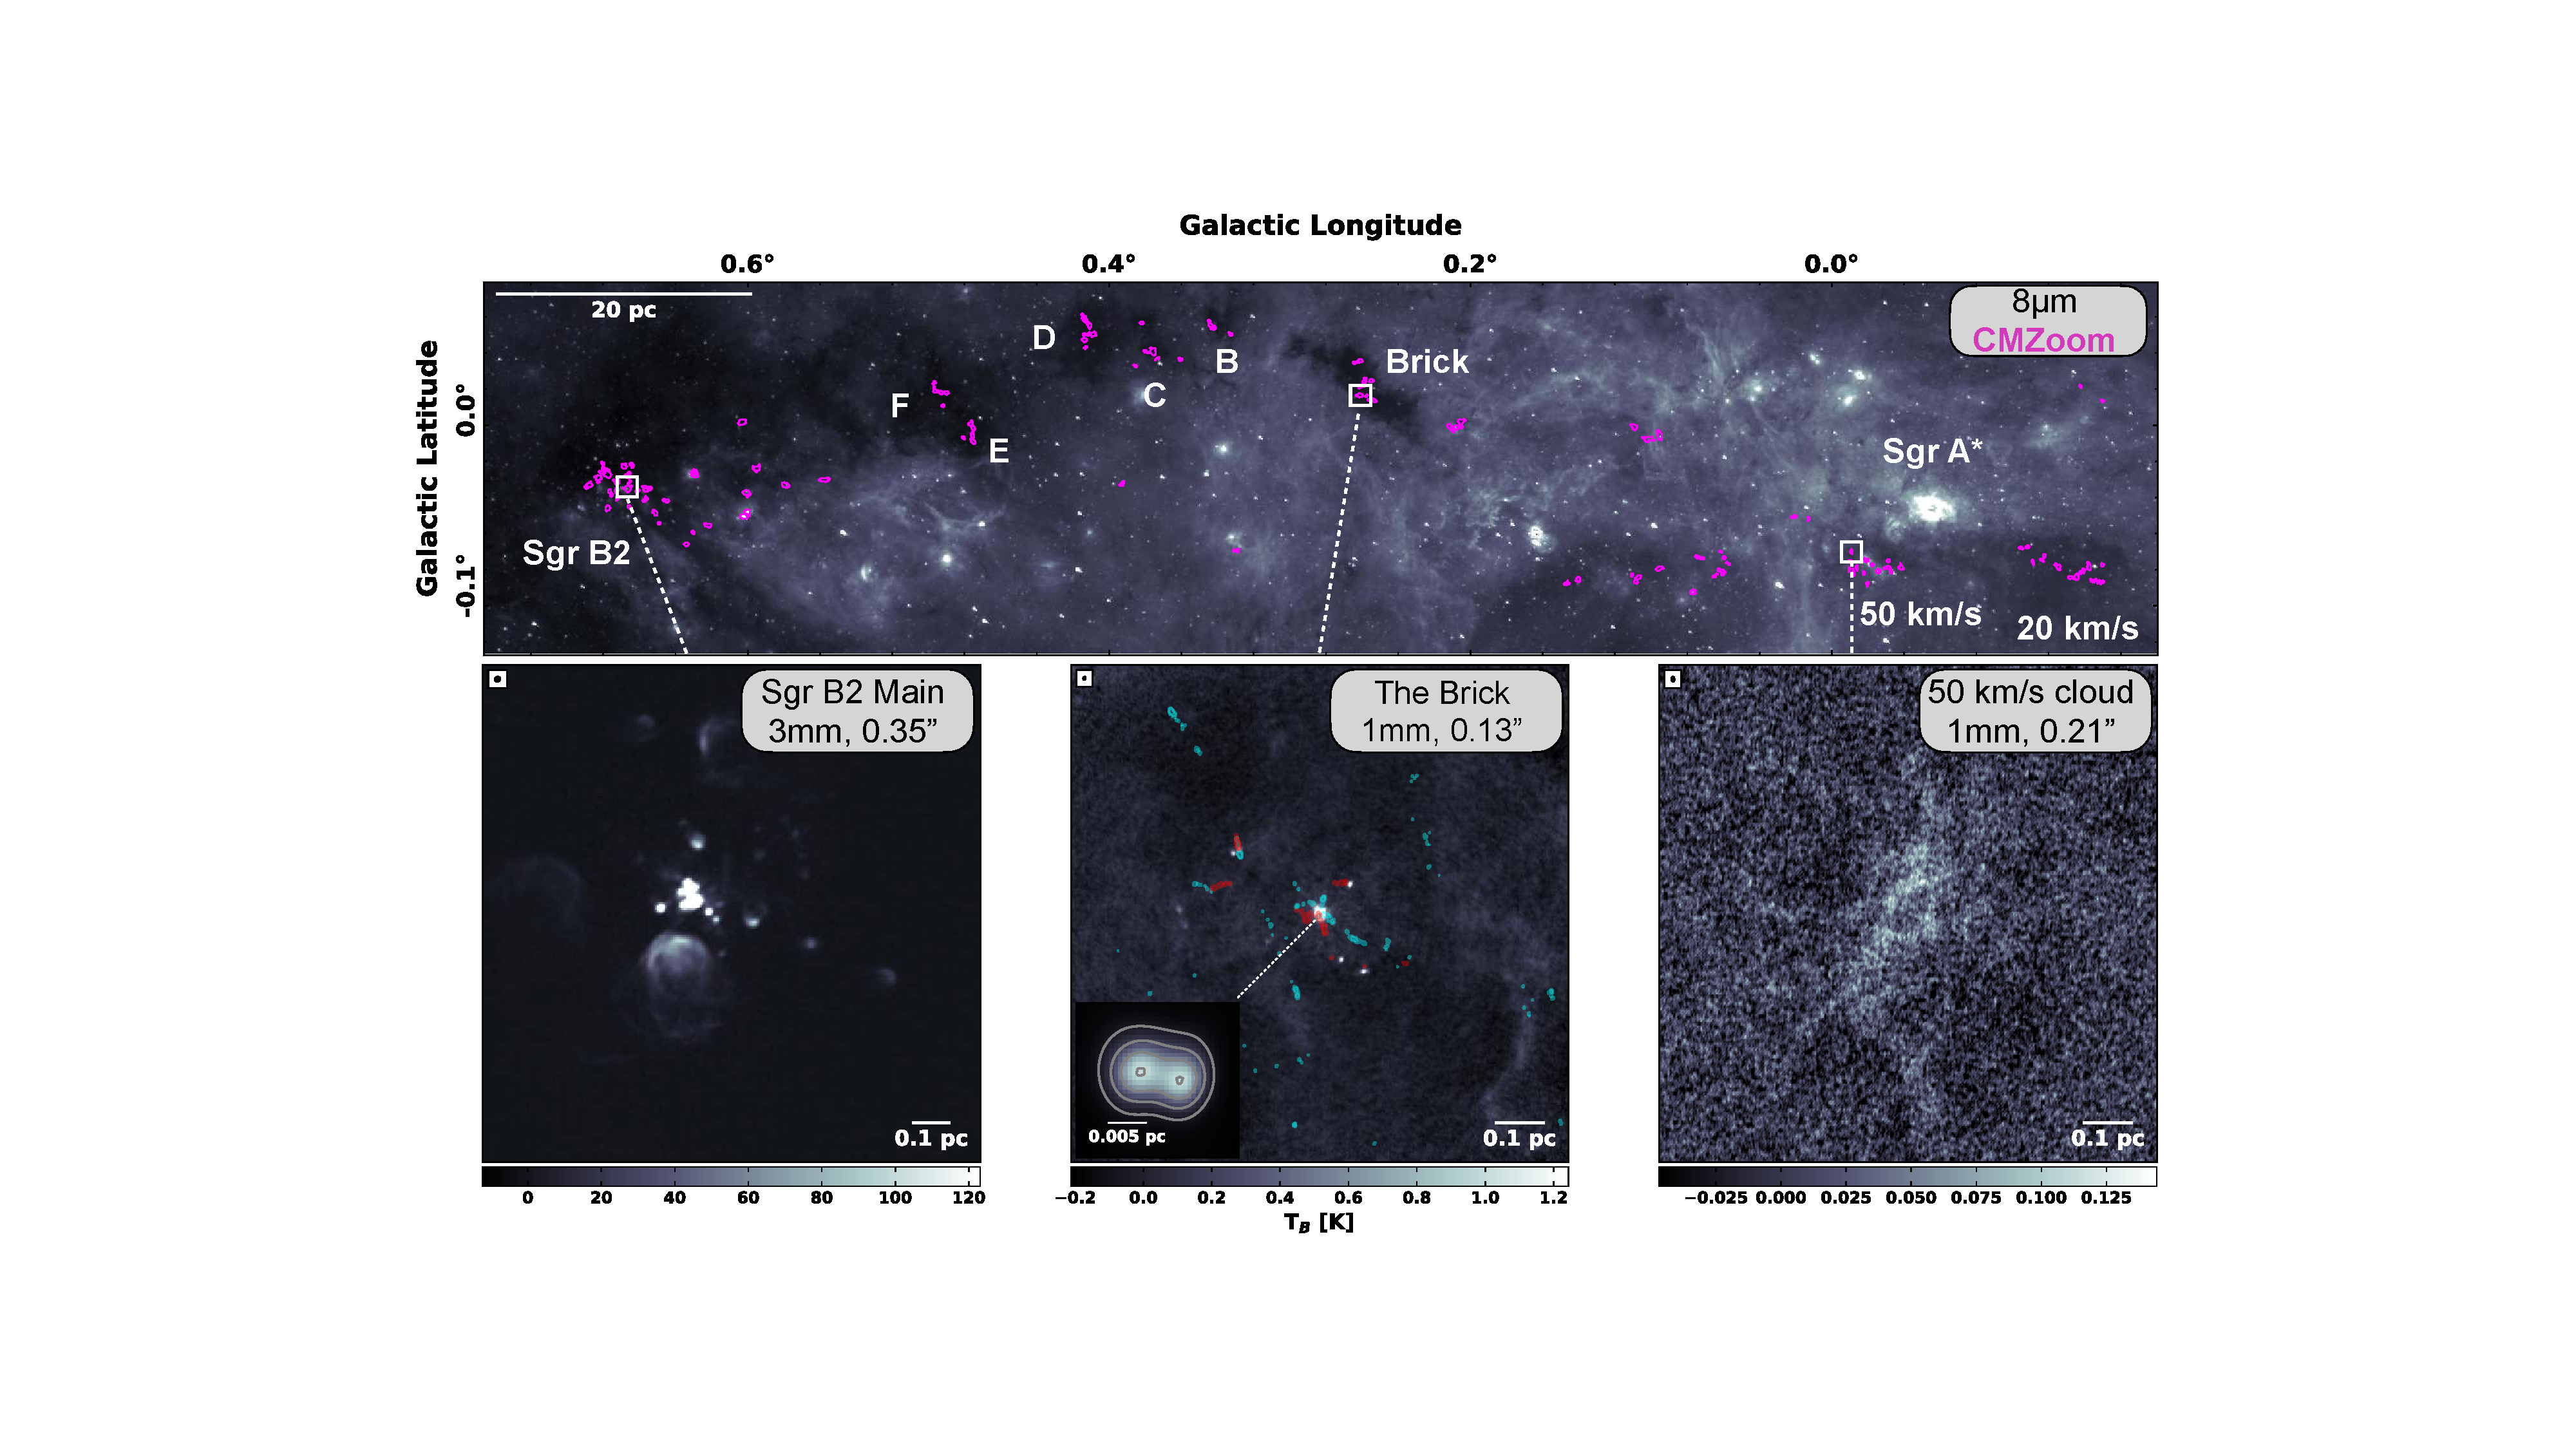
\includegraphics[trim=0 0cm 0 0cm, clip, width=0.95\textwidth]{./figs/high_res_colourbars_compressed.pdf}
    \caption{\textit{Top}: 8~$\mu$m map of a portion of the CMZ \citep{Churchwell2009}. Contours show the 1.3~mm source catalogue from the CMZoom survey \citep{Battersby2020}. \textit{Bottom}: ALMA observations of three regions with differing levels of star-forming activity: from the highly active Sgr B2 Main \citep[\textit{left},][]{Ginsburg2018b}, to the weakly star-forming G0.253+0.016 (the Brick) \citep[\textit{centre},][]{Walker2021}, and the 50~km~s$^{-1}$ cloud, which shows no evidence for embedded protostellar cores \citep[\textit{right},][]{Lu2020}. Blue/red contours in the centre panel show outflows via integrated blue/red-shifted SiO (5-4) emission, and the inset shows the the centre of the field, revealing a protostellar binary with separation $\sim$ 1000~AU.}
    \label{fig:high_res}
\end{figure*}

A crucial step in understanding the present-day star formation activity in the CMZ is the search for signposts of active star formation. Combined with the core populations discussed in $\S$\ref{sec:incipientsf}, these signatures (or lack thereof) provide key insights into their evolutionary phases, and ultimately a more comprehensive view of the overall SFR in the CMZ.

\paragraph{Masers:}\label{sec:masers} Maser emission\index{masers} is one of the most widely used tracers of early embedded star formation. Masers are particularly useful in the context of the CMZ, as their bright, compact emission signatures are more easily detectable through the complex, high-extinction line-of-sight compared to other star formation tracers. 

The two most abundant maser species found in star-forming regions are those from water (H$_{2}$O) and methanol (CH$_{3}$OH, Class II), with the latter being found exclusively towards regions of high-mass star formation \citep[e.g.][]{Ellingsen2006}. A number of Galactic plane surveys have obtained a census of these masers throughout the CMZ. The H$_{2}$O Southern Galactic Plane Survey \citep[HOPS,][]{Walsh2011} and the methanol multibeam survey \citep[MMB,][]{Green2009, Caswell2010} have surveyed the inner Galaxy for 22.2~GHz water masers and 6.7~GHz methanol masers, respectively. \citet{Walsh2011} reported an under-density of water masers in the CMZ given the amount of dense gas there as traced by NH$_{3}$ \citep{Longmore2013b}. 

\citet{Caswell2010} reported 22 methanol masers in the CMZ, 11 of which are in Sgr B2. More recently, \citet{Rickert2019} conducted a survey of 6.7~GHz methanol maser emission in the CMZ using the VLA, reporting a total of 43 masers. They note that there is an asymmetry about the Galactic centre, with more methanol masers at positive longitudes. This excess correlates with the asymmetry in the dense molecular gas in the CMZ, indicating more young high-mass star formation at positive longitudes (\S\ref{sec:gasstardistrib}). Similarly, \citet{Lu2019a} observed the 6.7~GHz methanol line over the inner 200~pc of the CMZ, reporting 23 methanol masers. Correlating these with embedded UC\hii\ regions, they find that high-mass star formation in the CMZ is limited to 7 clouds, with methanol masers detected towards only 5.
    
While the CMZ appears to be under-abundant in water and methanol masers, there is tentative evidence that it may be over-abundant in more exotic masers that trace high-mass star formation \citep{Ginsburg2015}. H$_{2}$CO masers, which appear to uniquely trace high-mass star formation, have been reported in Sgr B2, Sgr C, and dust ridge cloud C \citep{Ginsburg2015, Lu2019a}. This brings the total known Galactic star-forming regions containing H$_{2}$CO masers to 9, a third of which are in the CMZ. SiO masers have also been detected in Sgr B2 \citep{Higuchi2014} and dust ridge cloud C \citep{Ginsburg2015}. While SiO masers are common towards evolved stars, they are rare around YSOs, with 8 known high-mass star-forming regions, 2 of which are in the CMZ. $^{14}$NH$_{3}$ (2,2) maser emission has been detected in Sgr B2, which is the first reported detection in a star-forming region, and the eighth star-forming region known to contain an NH$_{3}$ maser \citep{Mills2018a}.  Additional masers from non-metastable lines of NH$_3$ have been found in Sgr B2 North \citep{Mei2020}. Though the sample is small, these results suggest that these rarer masers are more prevalent in the CMZ. The reason for this is unknown, but \citet{Ginsburg2015} speculate that either these masers trace very early stages of high-mass star formation, which would indicate that these regions are experiencing a burst of star formation, or that the comparatively extreme conditions in the CMZ could favour the production of masers.

\paragraph{Protostellar outflows:}\label{sec:outflows} Protostellar outflows\index{feedback!stellar!jets and outflows} are unambiguous signatures of star formation, indicating that the embedded YSO is actively accreting material. They have been ubiquitously observed both in regions of low- and high-mass star formation \citep[e.g.][and references therein]{Bally2016}. However, outflows in the CMZ have largely eluded detection until very recently. This is due to a previous lack of observations at high angular resolution and sensitivity, compounded by the kinematic complexity towards the CMZ, which makes it difficult to disentangle outflow emission. This is particularly true for the two most common outflow tracers, CO and SiO. Bright CO emission is widespread throughout the CMZ, and along the line-of-sight, resulting in absorption and complex spectra. SiO is also abundant in the gas-phase in the CMZ, likely due to turbulent shocks releasing it from grain surfaces \citep{Martin-Pintado1997}.

Until recently, the only candidate outflows in the CMZ were in Sgr B2 N and M \citep{Lis1993, Qin2008, Higuchi2014}. These outflows are extremely massive (10$^{2}$-10$^{3}$~M$_{\odot}$) and not well-collimated, and may instead represent a collective outflow from multiple high-mass protostars in the clusters (Schw\"{o}rer et al, private communication.).

With ALMA, it is now possible to resolve down to protostellar scales (\textless \ 1000~AU) at high enough sensitivity to isolate individual protostellar outflows in the CMZ. Recent ALMA observations probing these scales have unambiguously detected protostellar outflows in several CMZ clouds. \citet{Walker2021} reported at least 9 outflows in G0.253+0.016 (aka The Brick, see Fig.~\ref{fig:high_res}) as traced by SiO (5-4). \citet{Lu2021} reported a total of 43 outflows in 3 massive molecular clouds (Sgr C, Sgr B1-off, and the 20~km~s$^{-1}$ cloud) as traced by 6 different molecular lines at 1~mm (SiO, SO, CH$_{3}$OH, H$_{2}$CO, HC$_{3}$N, and HNCO). The outflows in these samples are detected towards both low- and high-mass cores. These results suggest that protostellar outflows are also ubiquitous in star-forming regions in the CMZ, and confirm that low- and high-mass star formation is occurring simultaneously in these clouds.

\paragraph{Protostars:}\label{sec:protostars} Hundreds of protostellar sources\index{protostars} have recently been discovered in the CMZ, with a growing census as facilities push to higher resolution and sensitivity. 

The `hot cores'\index{hot cores} of Sgr B2 N and M have been known for decades, and several new smaller hot cores were recently discovered \citep[e.g.][]{Sanchez-Monge2017, Bonfand2017, Bonfand2019}. Throughout the Sgr B2 cloud, there are $\gtrsim250$ high-mass protostellar cores \citep{Ginsburg2018b}, though the published data are very shallow and sensitive only to $M\gtrsim10$~\msun.

The 20 \kms\ cloud, the Sgr B1 ``off'' region (aka dust ridge clouds E/F), and Sgr C are all forming rich groups of 100s of stars, while the 50 \kms\ cloud, with a similar mass and overall density, is not \citep{Lu2020}. \citet{Uehara2019} identify a population `cores' from H$^{13}$CO$^{+}$ and C$^{34}$S data in the 50 \kms\ cloud, though \citet{Lu2020} found that there were no overdensities on 2000~AU scales in the 1~mm dust continuum that were consistent with protostellar sources. 

G0.253+0.016 contains only one known site of ongoing star formation, with 18 clustered protostars found so far. These protostars are all low mass, but the measured outflow rates of \textgreater\ $10^{-5}\mhyphen10^{-4}$~\msun~yr$^{-1}$ towards 50~\% of the sources suggests that they may be destined to become intermediate or high-mass stars \citep{Walker2021}. There is also some indirect evidence for on-going star formation in a different region of the cloud \citep{Henshaw2022}. The rest of G0.253+0.016 appears to be totally devoid of protostars, though it has not yet been fully mapped out at high angular resolution and sensitivity. These differences in protostellar activity between prominent CMZ clouds are highlighted in Figure \ref{fig:high_res}.

The populations of prestellar and protostellar cores in the CMZ have only been catalogued towards a handful of molecular clouds so far \citep[][Fig.~\ref{fig:high_res}]{Ginsburg2018b,Lu2020,Lu2021,Walker2021}. There is tentative evidence to suggest that the distribution of core masses -- the core mass function\index{core mass function} (CMF) -- is shallow: i.e. there is an apparent excess of high-mass sources (\citealp{Lu2020}, though the source mass function based on line data only by \citealp{Uehara2019}, with coarser resolution,  has a steeper distribution). However, there remain substantial uncertainties in these measurements; a `normal' Salpeter shape can still be accommodated if the dust temperature is systematically higher for the brighter cores \citep{Lu2020}. These initial results are similar to those found in CMZ star clusters, where there is some evidence that the stellar IMF is also top-heavy (\S\ref{sec:starclusters}).

Current observations show that searching for protostars based on the presence and number density of H$_{2}$O and CH$_{3}$OH masers (\S\ref{sec:masers})
has proved efficient for identifying sites of ongoing star formation.
Most of these clustered H$_{2}$O masers have proved to be closely associated with protostars or outflows \citep{Walker2021,Lu2021}. However, there are many molecular clouds that contain sufficient dense gas that we expect ongoing star formation, yet do not contain any known masers. Thus far, these clouds have only been systematically surveyed to a depth of $M_{\mathrm{core}}>10$~\msun at an angular resolution of 3\arcsec \citep{Battersby2020,Hatchfield2020}. A deep, high resolution, and complete survey is therefore needed to determine whether these apparently quiescent cloud host populations of low-to-intermediate mass protostars.

\paragraph{HII regions:}\label{sec:hiiregions}
The intense radiation field from high-mass (O- and B-type) stars produces regions of photoionised gas known as \hii regions\index{feedback!stellar!HII regions}, which, because of the short lifetimes of such stars, are treated as a sign of recent star formation.  

The Sgr B2 complex contains the majority of compact \hii\ regions in the CMZ, ranging in size from hundreds of AU to several pc (e.g. \citealp{Gaume1995, dePree1995, dePree1996}).
\citet{Schmiedeke2016} compiled a comprehensive list of \hii\ region surveys  in this cloud, and estimate a total stellar mass content of $\sim$2-3$\times$10$^4$\,\msun.
Short timescale flux variations of ultra-compact \hii\ (\uchii) regions in Sgr B2 highlight that accretion is still ongoing \citep{DePree2015}. 

Adjacent in projection to Sgr B2 is another notable \hii\ region complex: Sgr B1\index[obj]{Sagittarius B1} (Figure \ref{fig:rgb_main}). 
The Sgr B1 complex contains more diffuse ionised gas and less extincted infrared structure \citep{Mehringer1992}, consistent with it being at a later evolutionary stage than Sgr B2 (e.g. \citealp{Barnes2020b}).
\citet{Harris2021} argue for a physical association between Sgr B1 and B2 based on [CII] morphology.
Two scenarios have been proposed for the formation of this region: newly formed stars that are ionising their natal environment, or more evolved high-mass stars passing through, and ionising, the cloud.  
The maser emission \citep{Mehringer1993}, and YSO candidates identified towards this region (e.g \citealp{An2011,An2017}) point towards the former scenario. 
The latter scenario has been suggested by \citet{Simpson2018a, Simpson2021}, who suggest the ionising stars are several million years old based on ion line ratios. 
It is plausible that high-mass stars have drifted this far away from the nearby massive clusters \citep[][ \S\,\ref{sec:starclusters}]{Habibi2014}.
However, future tests of this hypothesis are needed, including investigating the proper motions and relative velocities of the ionised gas and stars, examining the structure of the molecular and ionised gas to search for cometary or bow-shock features \citep{Henshaw2022}, and age dating the embedded stellar populations (as in e.g. \citealp{Nogueras-Lara2020b}).

Near the projected centre of the CMZ are the Sgr A 20 \& 50 \kms\ clouds, which contain several \hii regions. \citet{Tsuboi2019} measure their recombination line emission, inferring electron temperatures $T_e\sim5000\mhyphen6000$ K, among the coolest in the Galaxy but consistent with other Galactic centre \hii regions \citep{Mills2011}.
The low electron temperatures are consistent with the high inferred metallicity in CMZ gas \citep{Balser2011}. The presence of these \hii regions is evidence for recent star formation in the 20 and 50 \kms clouds.

On the opposite side of the CMZ to Sgr B2 is the Sgr C complex (Figure~\ref{fig:rgb_main}), which contains more than $\sim$\,250\msun of ionised gas that powered by at least one O star (e.g. \citealp{Liszt1995}). To the east of the \hii\ region lies a dense molecular cloud with a mass $\sim$10$^5$\msun (e.g. \citealp{Lis1994b}), which is likely interacting with the ionised gas \citep{Lang2010}. \citet{Hankins2020} identified numerous bright mid-IR (37\micron) point sources on the boundary of the molecular cloud and \hii\ region that are candidate \uchii regions. The brightest of these is the Sgr C ``H3'' region, which has been confirmed as an \uchii region (e.g. \citealp{Forster2000, Kendrew2013, Lu2019a, Lu2019b}).

Just outside of the CMZ, there are \hii regions associated with infalling material, indicating that there is some ongoing star formation in the dust lanes.
In the far side dust-lane at negative longitudes (\S\,\ref{sec:dustlanes}), there is the Sgr E complex (e.g. \citealp{Liszt1992}). This region contains $\sim$\,60 \hii\ regions \citep{Anderson2020}, which are surrounded by a diffuse ionised gas component \citep{Langer2015}. These \hii\ regions are scattered across nearly a degree on the sky, are not centrally concentrated, and have relatively uniform sizes. Comparison with simulations suggests that the stars responsible for these \hii\ regions formed upstream in the far dust lane a few Myr ago and will overshoot the CMZ, crashing through the near dust lane in the future \citep{Anderson2020}.

While the compact \hii\ region population in the CMZ has been known and reasonably well-characterised for several decades, there have been several more recent discoveries of diffuse \hii\ regions (e.g. \citealp{Henshaw2022, Heywood2022}). This suggests that there is more to be learned through observational studies of these larger \hii\ regions and the recent ($3\mhyphen30$ Myr) star formation history of the CMZ.